%============================
% SECTION 3: VOLUME DATA STRUCTURE
%============================
\section{Volume Data Structure}

\begin{frame}
\frametitle{Volume Representation}

\textbf{Definition:} A 3D array of voxel values organized as:
$$\text{Volume}[z][y][x] = \text{pixel intensity}$$

\begin{itemize}
  \item \textbf{Dimensions}: width $\times$ height $\times$ depth
  \item \textbf{Spacing}: Physical distance between voxels
  \item \textbf{Storage}: Linear Float32Array (memory efficient)
  \item \textbf{Indexing}: $(x, y, z) \rightarrow \text{offset} = x + y \cdot W + z \cdot W \cdot H$
\end{itemize}

\vspace{0.5cm}

\textbf{Key Properties:}
\begin{itemize}
  \item width: Number of columns
  \item height: Number of rows
  \item depth: Number of slices
  \item spacing: [pixelSpacing.x, pixelSpacing.y, sliceThickness]
  \item data: Float32Array (normalized pixel values)
  \item minValue, maxValue: For windowing
\end{itemize}
\end{frame}

\begin{frame}[fragile]{Volume Construction: Memory Mapping}
To pass data to a \textbf{WebGL 3D Texture}, we must flatten our stack of 2D slices into a single 1D array.

\begin{block}{Indexing Formula}
The position of a voxel at $(x, y, z)$ in the linear buffer is:
\[ \text{Index} = (z \times \text{width} \times \text{height}) + (y \times \text{width}) + x \]
\end{block}

\begin{lstlisting}
// Allocate linear array for the entire volume
this.data = new Float32Array(
  this.width * this.height * this.depth
);

// z-plane offset in the 1D array
const planeOffset = z * this.width * this.height;
\end{lstlisting}

\vfill
\small \textit{Note: We use \texttt{Float32Array} to allow for Hounsfield Unit (HU) precision after normalization.}
\end{frame}

\begin{frame}[fragile]{Volume Construction: Normalization}
The final step, \texttt{computeMinMax()}, is critical for rendering contrast.

\begin{lstlisting}
computeMinMax() {
  let min = Infinity, max = -Infinity;
  for (let i = 0; i < this.data.length; i++) {
    const val = this.data[i];
    if (val < min) min = val;
    if (val > max) max = val;
  }
  this.stats = { min, max };
}
\end{lstlisting}

\begin{itemize}
    \item \textbf{Windowing:} Allows the user to focus on "Soft Tissue" vs "Bone".
    \item \textbf{GPU Ready:} Pre-calculating these bounds allows the shader to normalize values on the fly: $v_{norm} = \frac{v - min}{max - min}$.
\end{itemize}
\end{frame}

\begin{frame}[fragile]
\frametitle{Memory Layout: 3D to 1D Mapping}

\begin{center}
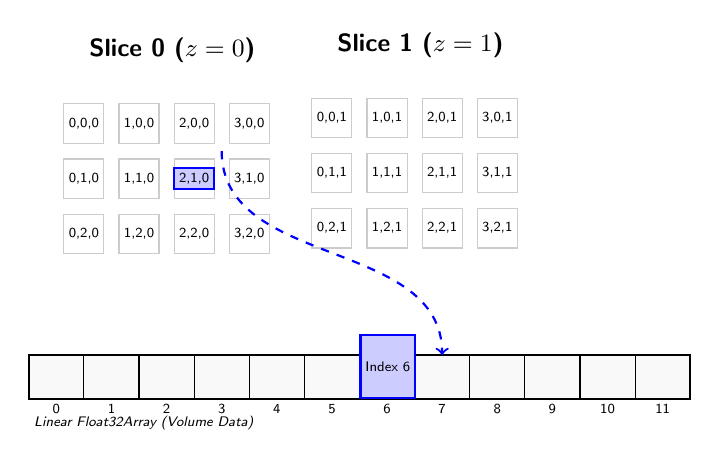
\begin{tikzpicture}[
    scale=0.7, 
    z={(0.5cm,0.4cm)}, % Custom 3D perspective
    node font=\tiny\sffamily,
    cell/.style={draw=black!20, fill=white, minimum size=0.5cm},
    highlight/.style={fill=blue!20, draw=blue, thick}
]

  % --- SLICE 1 (Back/z=1) ---
  \begin{scope}[shift={(2.5,-1.5,4)}]
    \node[anchor=south west, font=\bfseries\small] at (0,3) {Slice 1 ($z=1$)};
    \foreach \y in {0,...,2}
      \foreach \x in {0,...,3}
        \node[cell] (z1-\x-\y) at (\x,2-\y) {\x,\y,1};
  \end{scope}

  % --- SLICE 0 (Front/z=0) ---
  \begin{scope}[shift={(0,0,0)}]
    \node[anchor=south west, font=\bfseries\small] at (0,3) {Slice 0 ($z=0$)};
    \foreach \y in {0,...,2}
      \foreach \x in {0,...,3}
        \node[cell] (z0-\x-\y) at (\x,2-\y) {\x,\y,0};
        
    % Highlight a specific voxel: (2,1,0)
    \node[highlight] at (2,1) {2,1,0};
  \end{scope}

  % --- LINEAR ARRAY (Below) ---
  \begin{scope}[shift={(-1,-3,0)}]
    \draw[thick, fill=gray!5] (0,0) rectangle (12,0.8);
    \foreach \i in {0,...,11} {
        \draw (\i,0) -- (\i,0.8);
        \node[anchor=north] at (\i+0.5, 0) {\i};
    }
    % Highlight the mapped index: 2 + (1*4) + (0*12) = 6
    \node[highlight, minimum height=0.8cm, anchor=south west] at (6,0) {Index 6};
    \node[anchor=north west, font=\itshape] at (0,-0.2) {Linear Float32Array (Volume Data)};
  \end{scope}

  % Connection Arrow
  \draw[->, blue, thick, dashed] (2.5,1.5,0) [out=-90, in=90] to (6.5,-2.2,0);

\end{tikzpicture}
\end{center}

\begin{exampleblock}{The Mapping Formula}
\[ \text{Index} = x + (y \cdot W) + (z \cdot W \cdot H) \]
\textbf{Calculation:} For $V(2,1,0) \rightarrow 2 + (1 \cdot 4) + (0 \cdot 12) = \mathbf{6}$
\end{exampleblock}

\end{frame}